\chapter{耦合径流模型的产流和汇流过程}

\section{产流参数化方案}
%\addcontentsline{toc}{chapter}{陆地表面的水分循环}

\subsection{地表产流}
\begin{mymdframed}{代码}
  本节对应的代码文件为\texttt{MOD\_SoilSnowHydrology.F90}。
\end{mymdframed}
\subsubsection{基于SIMTOP参数化方案}
地表径流的参数化方案~\citep{niu2005simple}考虑了地形、地下水位、降水和入渗速度等因素。

模式网格内饱和区域的面积$f_{\mathrm{sat}}$通过以下方案估算,
\begin{equation}
  f_{\mathrm{sat}}=f_{\mathrm{wt}}  \mathrm{e}^{-0.5  f_{\mathrm{decay}}  z_{\mathrm{wt}}}
\end{equation}
其中,$f_{\mathrm{wt}}$为最大饱和面积(模式中取固定值0.38,为全球平均),$f_{\mathrm{decay}}$为径流的衰减因子(模式中取固定值0.5),$z_{\mathrm{wt}}$为地下水位 (m)。

最大入渗能力的计算考虑了最上面三层土壤的物理状态和属性,
\begin{equation}
  q_{\mathrm{infl}, \max }= \min _{i=1,2,3} 10^{-6.0  f_{\mathrm{ice}, i}}  K_{\mathrm{sat}, i}
\end{equation}
其中,$f_{\mathrm{ice},i}$表示第$i$层中冰占土壤孔隙的体积百分比,$K_{\mathrm{sat},i}$表示第$i$层的饱和导水率。

假设到达地表的净水流通量为$G_{\mathrm{wat}}$。 一个模式计算单元内,饱和区域的地表水全部转化为径流流走,非饱和区域的地表水,部分入渗到土壤中,剩余部分转化为径流,总的地表径流$r_{\rm sur}$为:
\begin{equation}
  r_{\mathrm{sur}}=f_{\mathrm{sat}} G_{\mathrm{wat}}+\left(1-f_{\mathrm{sat}}\right)  \left(G_{\mathrm{wat}}-q_{\mathrm{infl},\max}\right)
\end{equation}
入渗到土壤中的部分等于输入的净水流通量减去地表径流,即
\begin{equation}
  q_{\mathrm{infl}}={G}_{\mathrm{wat}}-r_{\mathrm{sur}}
\end{equation}
\subsubsection{基于新安江模型的地表产流方案}

\subsubsection{基于Simple-VIC的地表产流方案}
\cite{Liang2003Anew}提出的这一参数化方案充分考虑了土壤的物理特性,包括土壤质地、饱和程度和水分深度等关键因素。该方案首先计算土壤的最大入渗能力,我们首先假设最大入渗能力取决于最上面6层土壤的物理状态和属性,即:
\begin{equation}
w_{{int}} = \sum_{i=1}^{6}\left( {vol}_{i} \times {dz}_{i} \right)
\end{equation}
\begin{equation}
w_{{satint}} = \sum_{i=1}^{6}\left( {eff}_{i} \times {dz}_{i} \right)
\end{equation}
其中,$w_{{int}}$ 表示前6层土壤中的液态水体积,$w_{{satint}}$ 表示前6层土壤中的饱和水体积。 ${dz}_{i}$ 表示第 $i$ 层土壤厚度, ${vol}_{i}$ 表示第 $i$ 层土壤中液态水体积百分比,${eff}_{i}$ 表示第 $i$ 层有效孔隙度。由此我们可以计算得出土壤饱和分数:
\begin{equation}
{S}_{{Sf}} = 1 - \left( 1 - \frac{w_{{int}}}{w_{{satint}}} \right)^{{I}_{{ef}}}
\end{equation}
其中,${I}_{{ef}}$ 为渗透指数因子:
\begin{equation}
{I}_{{ef}} = \frac{B_{{VIC}}}{1 + B_{\text{VIC}}}
\end{equation}
入渗参数~$B_{{VIC}}$~是用于表示土壤饱和比例的参数,数值介于0-1,其具体取值与Noah-MP保持一致,即由USDA定义的土壤分类计算得来,其主要特性在于随着土壤中的石英含量越高,~$B_{VIC}$~的取值越接近于1。土壤层初始和最大水深计算如下:
\begin{equation}
z_{\mathrm{wt,max}}= \left( 1 + B_{{VIC}} \right) \times w_{{satint}}
\end{equation}
\begin{equation}
z_{\mathrm{wt,init}} = z_{\mathrm{wt,max}} \times \left( 1 - \left( 1 - {S}_{{sf}} \right)^{\frac{1}{B_{{VIC}}}} \right)
\end{equation}
假设到达地表的净水流通量为$G_{\mathrm{wat}}$,则该方案的地表产流$r_{\mathrm{sur}}$考虑三种情况:
\begin{equation}
r_{\mathrm{sur}} = 
\begin{cases}
G_{\mathrm{wat}} & \text{当 } z_{\mathrm{wt,max}} \leq 0 \\
G_{\mathrm{wat}} - w_{{satint}} + w_{{int}} & \text{当 } z_{\mathrm{wt,init}} + G_{\mathrm{wat}} > z_{\mathrm{wt,max}} \\
G_{\mathrm{wat}}- w_{{satint}} + w_{{int}} + w_{{satint}} \times {{I}_{{tmp}}}^{1 + B_{{VIC}}} & \text{其他情况}
\end{cases}
\end{equation}
其中:
\begin{equation}
{I}_{tmp} = 1 - \frac{\left( z_{\mathrm{wt,init}} + {G}_{\mathrm{wat}} \right)}{z_{\mathrm{wt,max}}}
\end{equation}
最后,入渗量$q_{\mathrm{infl}}$由净水流通量和地表产流量决定:
\begin{equation}
  q_{\mathrm{infl}}={G}_{\mathrm{wat}}-r_{\mathrm{sur}}
\end{equation}






\subsection{地下产流} \label{section:rsub_par}
\begin{mymdframed}{代码}
  本节对应的代码文件为\texttt{MOD\_SoilSnowHydrology.F90}。
\end{mymdframed}

地下产流的大小与地形和地下水位有关\citep{niu2005simple},
\begin{equation}
  r_{\mathrm{sub}} = r_{\mathrm{sub,max}} \exp \left(-f_{\mathrm{drai}}  z_{\mathrm{wt}}\right)
\end{equation}
其中,$r_{\mathrm{sub,max}}$为产流的最大值,取决于地形坡面的大小,
模式中取全球统一的数值$5.5\times 10^{-3}~\unit{mm~s^{-1}}$;$f_{\mathrm{drai}}=2.5$ \unit{m^{-1}} 为衰减因子。

当土壤中含有冰时,需考虑冰对地下径流的阻力作用,
\begin{equation}
  \begin{aligned}
    f_{\mathrm{impd,ice}} & = 1 - \frac{\exp \left[-3 \left(1-f_{\mathrm{ice,sum}}\right)\right]
    -\exp (-3)}{1-\exp (-3)} \\
    r_{\mathrm{sub}} & = f_{\mathrm{impd,ice}}  r_{\mathrm{sub,max}}
    \exp \left(-f_{\mathrm{drai}}  z_{\mathrm{wt}}\right)
  \end{aligned}
\end{equation}
其中,$f_{\mathrm{ice,sum}}$为地下水位所在及以下土壤层内总的冰的体积含量(定义为冰的总体积除以土壤层的总体积)。

\subsection{其它可选产流方案}
\begin{mymdframed}{代码}
  本节对应的代码文件为\texttt{MOD\_Hydro\_VIC.F90}、\texttt{MOD\_Hydro\_VIC\_Variables.F90}。
\end{mymdframed}

CoLM2024进一步耦合了VIC模型的产流方案,作为产流计算的可选方案。VIC(Variable Infiltration Capacity,“可变下渗容量模型”)是基于~\citet{liang1994simple} 的思想研制出的大尺度分布式水文模型。\citet{liang1994simple} 等人将VIC-2L模型的上层分出一个顶薄层,而成为3层。VIC模型的地表径流和基流分别在不同的土壤层中计算。上方两层土壤产生径流,而最下层土壤产生基流。

\begin{enumerate}
  \item 地表径流

    VIC模型基于土壤可变下渗能力曲线进行地表径流的计算。当降水量大于土壤下渗能力时,其计算公式为:
    \begin{equation}
      Q_d\cdot\Delta t=
      \begin{cases}
        P\cdot\Delta t - W_1^c + W_1^-, & i_0 + P\cdot\Delta t \geqslant i_m \\
        P\cdot\Delta t - W_1^c + W_1^- + W_1^c \left(1-\frac{i_0+P\cdot\Delta t}{i_m} \right)^{1+b}, & i_0 + P\cdot\Delta t \leqslant i_m
      \end{cases}
    \end{equation}
    其中, $Q_d$ 为地表径流,$P$ 为降雨量,$i_0$ 为时段初的土壤下渗能力, $i_m$ 为土壤的最大下渗能力,$W_1^-$ 为时段初的土壤总含水量, $W_1^c$ 为土壤的最大蓄水容量,其计算公式为:
    \begin{equation}
      W_1^c = \frac{i_m}{1+b}
    \end{equation}
    其中 $b$ 为下渗能力曲线的形状参数。

    水量平衡方程式如下:
    \begin{equation}
      W_1^+ = W_1^- + (P - Q_d - Q_{12} - E_1)\cdot\Delta t,
    \end{equation}
    其中 $W_1^+$ 为土壤时段末的含水量, $Q_{12}$ 代表时段内由于重力作用从第二层到第三层土壤的下渗量,$E_1$ 为上两层土壤的蒸发量。$Q_{12}$ 计算公式为:
    \begin{equation}
      Q_{12} = K_s \left(\frac{W_1-\theta_r}{W_1^c-\theta_r}\right)^{\frac{2}{B_p} + 3},
    \end{equation}
    式中 $\theta_r$ 为土壤残留水分,$K_s$ 为饱和渗透系数,$B_p$ 为土壤孔隙大小分布指数。

  \item 基流

    在VIC模型中,基流仅在第三层土壤中形成,应用 Arno 概念模型计算基流:
    \begin{equation}
      Q_b = 
      \begin{cases}
        \frac{D_s D_m}{W_s W_2} W_2^-, & 0 \leqslant W_2^- \leqslant W_s W_2^c \\
        \frac{D_s D_m}{W_s W_2} W_2^- + \left(D_m - \frac{D_s D_m}{W_s}\right) \left(\frac{W_2^--W_s W_2^c}{W_2^c-W_s W_2^c}\right)^2,  & W_2^- \geqslant W_s W_2^c
      \end{cases}
    \end{equation}
    其中,$Q_b$ 为基流量,$D_m$ 是最大日基流量,$D_s$ 是占最大日基流量的比例,$W_2^-$ 是初始时段的下层土壤含水量,$W_2^c$ 是下层土壤的最大含水量,$W_s$ 是占 $W_2^c$ 的比例值,满足 $D_s\leqslant W_s$。下层土壤的水量平衡方程为式:
    \begin{equation}
      W_2^+ = W_2^- + (Q_{12} - Q_b -E_2)\cdot\Delta t,
    \end{equation}
    式中,$W_2^+$ 为最下层土壤时段末的含水量,$E_2$ 为最下层土壤的蒸发量。

  \item 方案可率定参数

    决定VIC大尺度水文模型模拟精确度的因素中,除了模型对各个水文过程的精确考虑和详细表达外,最重要的就是对模型参数的最优化选取,即模型参数的率定。VIC模型径流模拟中需要对以下四个参数进行率定(见表~\ref{tab:VIC率定参数}):
    \begin{enumerate}
      \item 可变下渗曲线参数 $b$,$b$ 增大时会减少下渗量,从而使得模拟的洪峰值增大,取值范围一般为 $0-0.4$ 之间。
      \item 最大基流流速 $D_m$,与土壤水力传导度有关,一般取值范围为 $1-30$。
      \item 非线性基流开始时基流值与最大基流值的比值 $D_s$,该值会影响基流,$D_s$ 增大会增加模拟的径流。$D_s$ 与年干燥度呈负相关,一般取值范围为 $0-1$。
      \item 非线性基流开始时第三层土壤含水量占最大土壤含水量的比值 $W_s$,$W_s$ 值越大将推迟洪峰出现的时间,一般取值范围为 $0-1$。
    \end{enumerate}
    {
      \begin{table}[htbp]
        \centering \renewcommand{\arraystretch}{1.5}
        \caption{VIC率定参数}
        \begin{tabular}{ccp{12cm}}
          \toprule
          参数  & 范围    & 含义                                                                                                                                   \\ \midrule
          $b$   & $0-0.4$ & 下渗能力曲线形状参数。数值越大下渗越小,$Q_d$ 越大                                                                                     \\
          $D_m$ & $0-30$  & 最底层土壤能产生的最大基流,与土壤水力传导度有关                                                                                       \\
          $D_s$ & $0-1$   & 基流出现快速非线性增长时占 $D_m$ 的比例。数值越大,$Q_b$ 越大                                                                          \\
          $W_s$ & $0-1$   & 基流出现快速非线性增长时底层土壤含水量占该层最大土壤含水量的比例。$W_s$ 值越高,快速增加的非线性基流所需的含水量就越高,将延迟径流峰值 \\
          \bottomrule
        \end{tabular}
        \label{tab:VIC率定参数}
      \end{table}
    }

  \item VIC与CoLM耦合

    VIC向CoLM传入的变量有土壤层厚度(\texttt{dz\_soi})、土壤孔隙度(\texttt{porsl})、残余水分含量(\texttt{theta\_r})、饱和导水率(\texttt{hksati})、Clapp-Hornberger参数 $b$(\texttt{bsw})、土壤层中液态水含量(\texttt{wliq\_soisno})、土壤层中固态水含量(\texttt{wice\_soisno})、根系从每层土壤中的吸水速率(\texttt{rootflux})和从冠层到大气的蒸散发(\texttt{fevpg})。VIC 向 CoLM 返回的变量有地表径流(\texttt{rsur})和基流(\texttt{rsubst})。

    VIC中的三层土壤和 CoLM 中的1--3、4--6、7--10层分别进行对应(见图~\ref{fig:VIC和CoLM耦合示意图} 所示)。对变量值做直接加和或者以土壤厚度作为权重进行加权平均。

    {
      \begin{figure}[htbp]
        \centering
        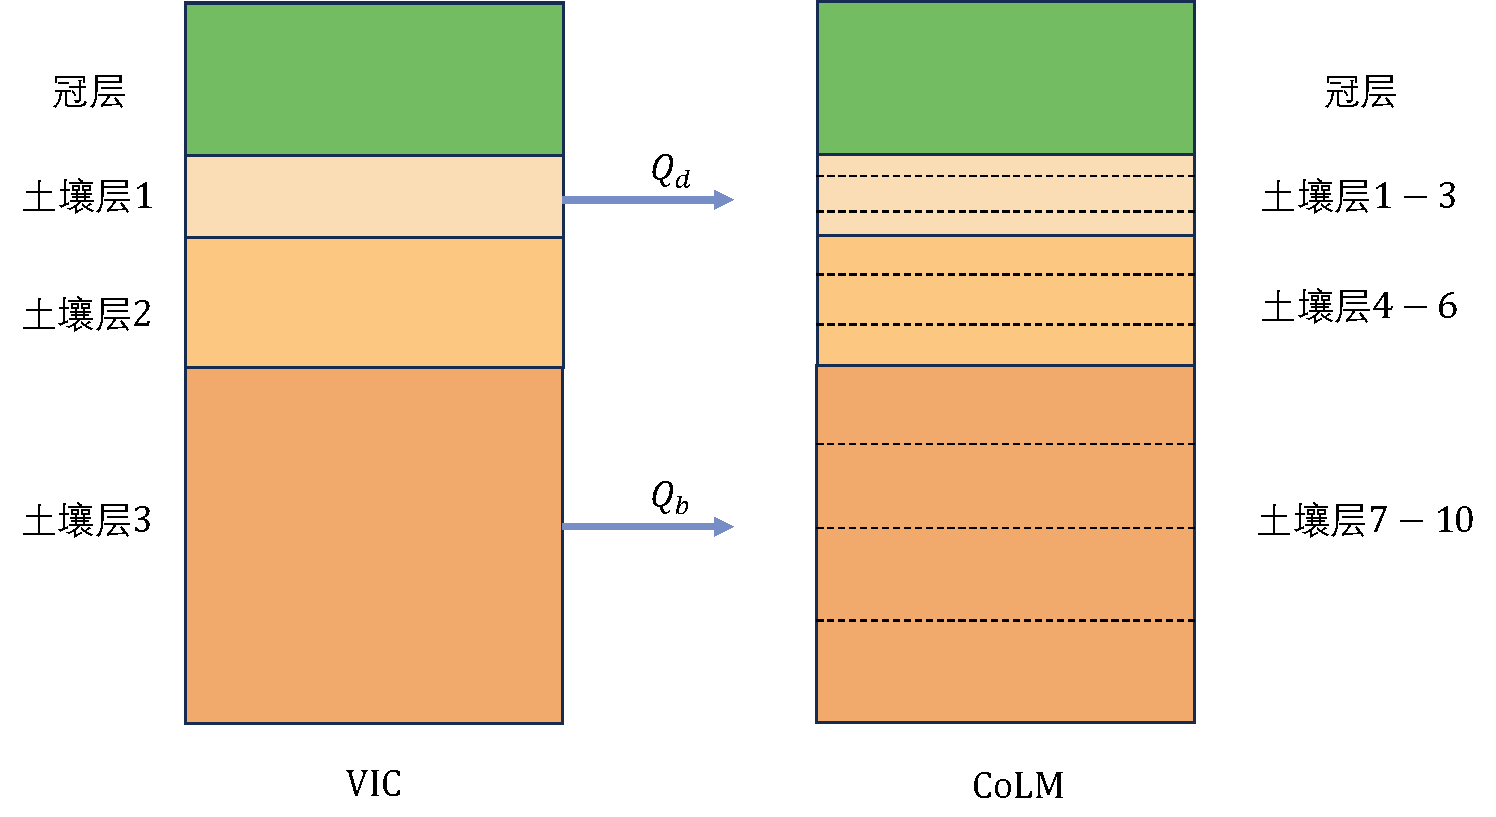
\includegraphics[width=\textwidth]{Figures/陆地表面的水分循环/VIC说明图中文.pdf}
        \caption{VIC和CoLM耦合示意图}
        \label{fig:VIC和CoLM耦合示意图}
      \end{figure}
    }
\end{enumerate}

\section{径流模型CaMa-Flood}
%\addcontentsline{toc}{chapter}{陆地表面的水分循环}
\begin{mymdframed}{代码}
  本节对应的代码文件夹为\texttt{CaMa/src},\\具体关联文件为\texttt{CaMa/src/MOD\_CaMa\_colmCaMa.F90}。
\end{mymdframed}

汇流计算是通过耦合 Dai Yamazaki 等人于2011年提出的大尺度分布式汇流模型 CaMa-Flood (Catchment-based Macro-scale Floodplain) 实现的\citep{yamazaki2011physically}。CaMa-Flood将全球河流网络分割为称为流域单元 (unit catchment) 的水文单元,在各单元集水区内利用河道 (river channel) 和漫滩 (floodplain) 的次网格 (subgrid) 地形参数以及陆面模式生成的产流量 (total runoff),对总蓄水量 (total storage) 以及总流量 (total discharge) 进行预测。
该模型进一步实现对河道及漫滩流量 (river discharge and flood discharge),漫滩面积 (flood area) 以及平均漫滩水深 (flood depth) 等日常所需的诊断量的高速计算。总蓄水量和总流量的时间演变通过求解局部惯性方程 \citep{bates2010} 得出。CaMa-Flood同时考虑了上游单元的入流、下游单元的流出和每个流域单元的径流强迫输入,是目前高速求解河道水动力方程-圣维南方程最为高速有效的方法之一。


CaMa-Flood 模型的主要优势之一在于除了能够精确描述河道径流以外,还能够模拟包括漫滩水位和漫滩面积变化等洪泛过程。因此,对模拟结果的验证不仅仅局限于传统测量河流流量,还可以直接将模拟结果与卫星高度计对水面高程的观测以及微波成像仪对洪泛面积的估算进行比较;这种多元验证方法能够有效加强全球河流模型各个输出的校准/验证\citep{yamazaki2012adjustment,yamazaki2012analysis}。
CaMa-Flood 模型的另一个优势在于它具有极高的模拟计算效率。通过引入次网格地形参数,复杂的漫滩淹没物理过程被合理地简化。与此同时,通过实现局部惯性方程和自适应时间步长等物理方案\citep{bates2010},河流流量和蓄水量的预测计算成本得到压缩,有利于进行集成/长期实验等计算要求高的实验或者与陆面模式之间的动态耦合。


关于CaMa-Flood模型的详细描述可以从相关文献获取\citep{yamazaki2011physically,yamazaki2013improving,yamazaki2014regional,yamazaki2014development}。目前耦合版本陆面过程模式分系统已经包含 CaMa-Flood v4.21 版本,并保持同步更新。

\subsection{诊断洪泛状态}\label{诊断洪泛状态}
在 CaMa-Flood 中指定网格的漫滩 (洪泛) 状态是通过计算该网格的蓄水总量得出的。如图~\ref{fig:CaMa-Flood流域单位示意图}
所示,河流河道蓄水量$S_{\mathrm {r}} $,漫滩蓄水量$S_{\mathrm {f}} $,河道水深度$D_{\mathrm {r}} $, 漫滩淹没深度$D_{\mathrm {f}} $,漫滩面积$A_{\mathrm {f}} $等均通过求解基于总蓄水量的水量方程得出。
首先,模式中引发当前流域单元洪水蓄水量$S_{\mathrm{ini}}$由如下公式进行确定:
\begin{equation}
  S_{\mathrm{ ini }}=B WL
\end{equation}
其中$B$是河道深度,$W$是河道宽度,及$L$是河道长度。如果总蓄水量$S$小于等于引发洪水蓄水量$S_{\mathrm{ini}}$,
CaMa-Flood 假设不存在漫滩 (洪泛) 事件,上述参数则通过如下方程计算得出:
\begin{equation}
  \begin{array}{l}S_{\mathrm {r}} =S \\ D_{\mathrm {r}} =\frac{S_{\mathrm {r}} }{WL} \\ S_{\mathrm {f}} =0 \\ D_{\mathrm {f}} =0 \\ A_{\mathrm {f}} =0 \end{array}
\end{equation}
当总蓄水量$S$大于引发洪水蓄水量$S_{\mathrm{ini}}$时,触发漫滩 (洪泛) 事件,则上述参数通过联立如下方程计算得出:
\begin{equation}
  \begin{aligned}
    S_{\mathrm {r}}  &=S-S_{\mathrm {f}}  \\
    D_{\mathrm {r}}  &=\frac{S_{\mathrm {r}} }{W L} \\
    S_{\mathrm {f}}  &=\int_{0}^{A_{\mathrm {f}} }[D_{\mathrm {f}} -D(A)]\,\mathrm{d}A  \\
    D_{\mathrm {f}}  &=D_{\mathrm {r}} -B \\
    A_{\mathrm {f}}  &=D^{-1}(D_{\mathrm {f}} )
  \end{aligned}
\end{equation}
上式中的$D_{\mathrm {f}}  = D_{\mathrm {r}}  - B$表示河道与漫滩的水面高度相同。该方程是基于河道与漫滩之间的水量瞬间完成交换的假设。
函数$D^{-1}(D_{\mathrm {f}} )$是漫滩高程剖面$D(A_{\mathrm {f}} )$的反函数,它将泛滥地区$A_{\mathrm {f}} $描述为漫滩水深$D_{\mathrm {f}} $的函数 (见图~\ref{fig:CaMa-Flood流域单位示意图})。


{
  \begin{figure}[htbp]
    \centering
    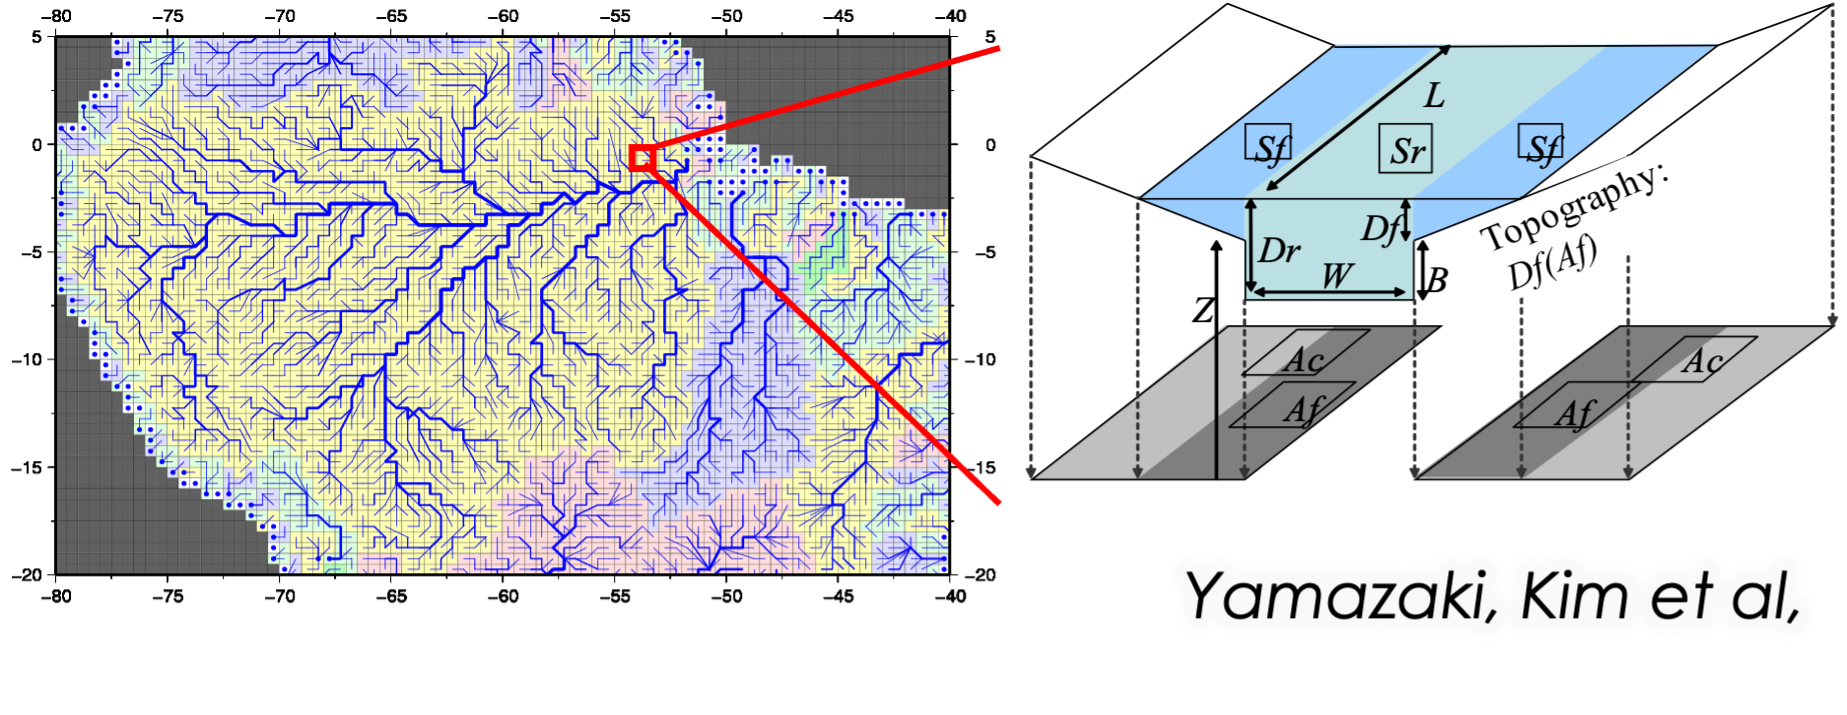
\includegraphics[width=\textwidth]{Figures/陆地表面的水分循环/CaMa-Flood流域单位示意图.png}
    \caption{CaMa-Flood流域单位示意图}
    \label{fig:CaMa-Flood流域单位示意图}
  \end{figure}
}

\subsection{河道径流流量计算}
CaMa-Flood 分别计算了各流域单元向其下游单元的河流径流量和漫滩流量。
二者的计算均通过忽略如下 St. Venant 动量方程式第二项,得到径流计算所使用的局部惯性方程~\citep{bates2010}:
\begin{equation}
  \frac{\partial Q}{\partial t}+\frac{\partial}{\partial x}\left[\frac{Q^{2}}{A}\right]+\frac{{\mathrm g} A \partial(h+z)}{\partial x}+\frac{{\mathrm g} n^{2} Q^{2}}{R^{4 / 3} A}=0
\end{equation}
式中$Q$为河流流量 (\unit{m^3.s^{-1}}),$A$为水流横截面面积 (\unit{m^2}),$h$为水流深度 (m),$z$为河床高程 (m),
$R$为水力半径 (m),$\rm g$为重力加速度 (\unit{m.s^{-2}}),$n$为曼宁摩擦系数(\unit{m^{-1/3}.s^{-1}})。
$x$和$t$分别为流动距离和时间。第一项、第二项、第三项和第四项分别表示局部加速度、平流、水面坡度和摩擦坡度。CaMa-Flood模型采用局部惯性方程的显式形式:
%
\begin{equation}
  Q^{t+\Delta t}=\frac{Q^{t}+\Delta t {\mathrm g} AS}{1+\frac{\Delta t {\mathrm g} n^{2}\left|Q^{t}\right|}{R^{4 / 3} A}}
\end{equation}
其中$S$是水面坡度,$Q^t$为当前时刻的流量, $Q^{t+\Delta t}$是单位时间间隔 $\Delta t$ 之后的流量。水力半径 $R$ 近似为水流深度。曼宁系数默认设置为$n=0.03$。
在局部惯性方程计算中可能出现的负向河流量,代表了下游流域单元向当前流域单元的反向水流(回水)。同时为防止当前网格的总的流出量超过蓄水量,
CaMa-Flood 引入限流器的概念:当总出水量大于网格的总库存量时,CaMa-Flood 使用修正系数对径流流量进行修正。


\subsection{洪水漫滩流量计算}
漫滩流量计算与河道径流流量计算方法相同。
其区别在于漫滩流量包括所使用的水流面积$A$的计算方法是漫滩蓄水量除以河道长度;
水流深度$h$为漫滩深度;漫滩流量的曼宁系数被设置为$n=0.10$。


\subsection{蓄水量变化计算}
{
  \begin{figure}[htbp]
    \centering
    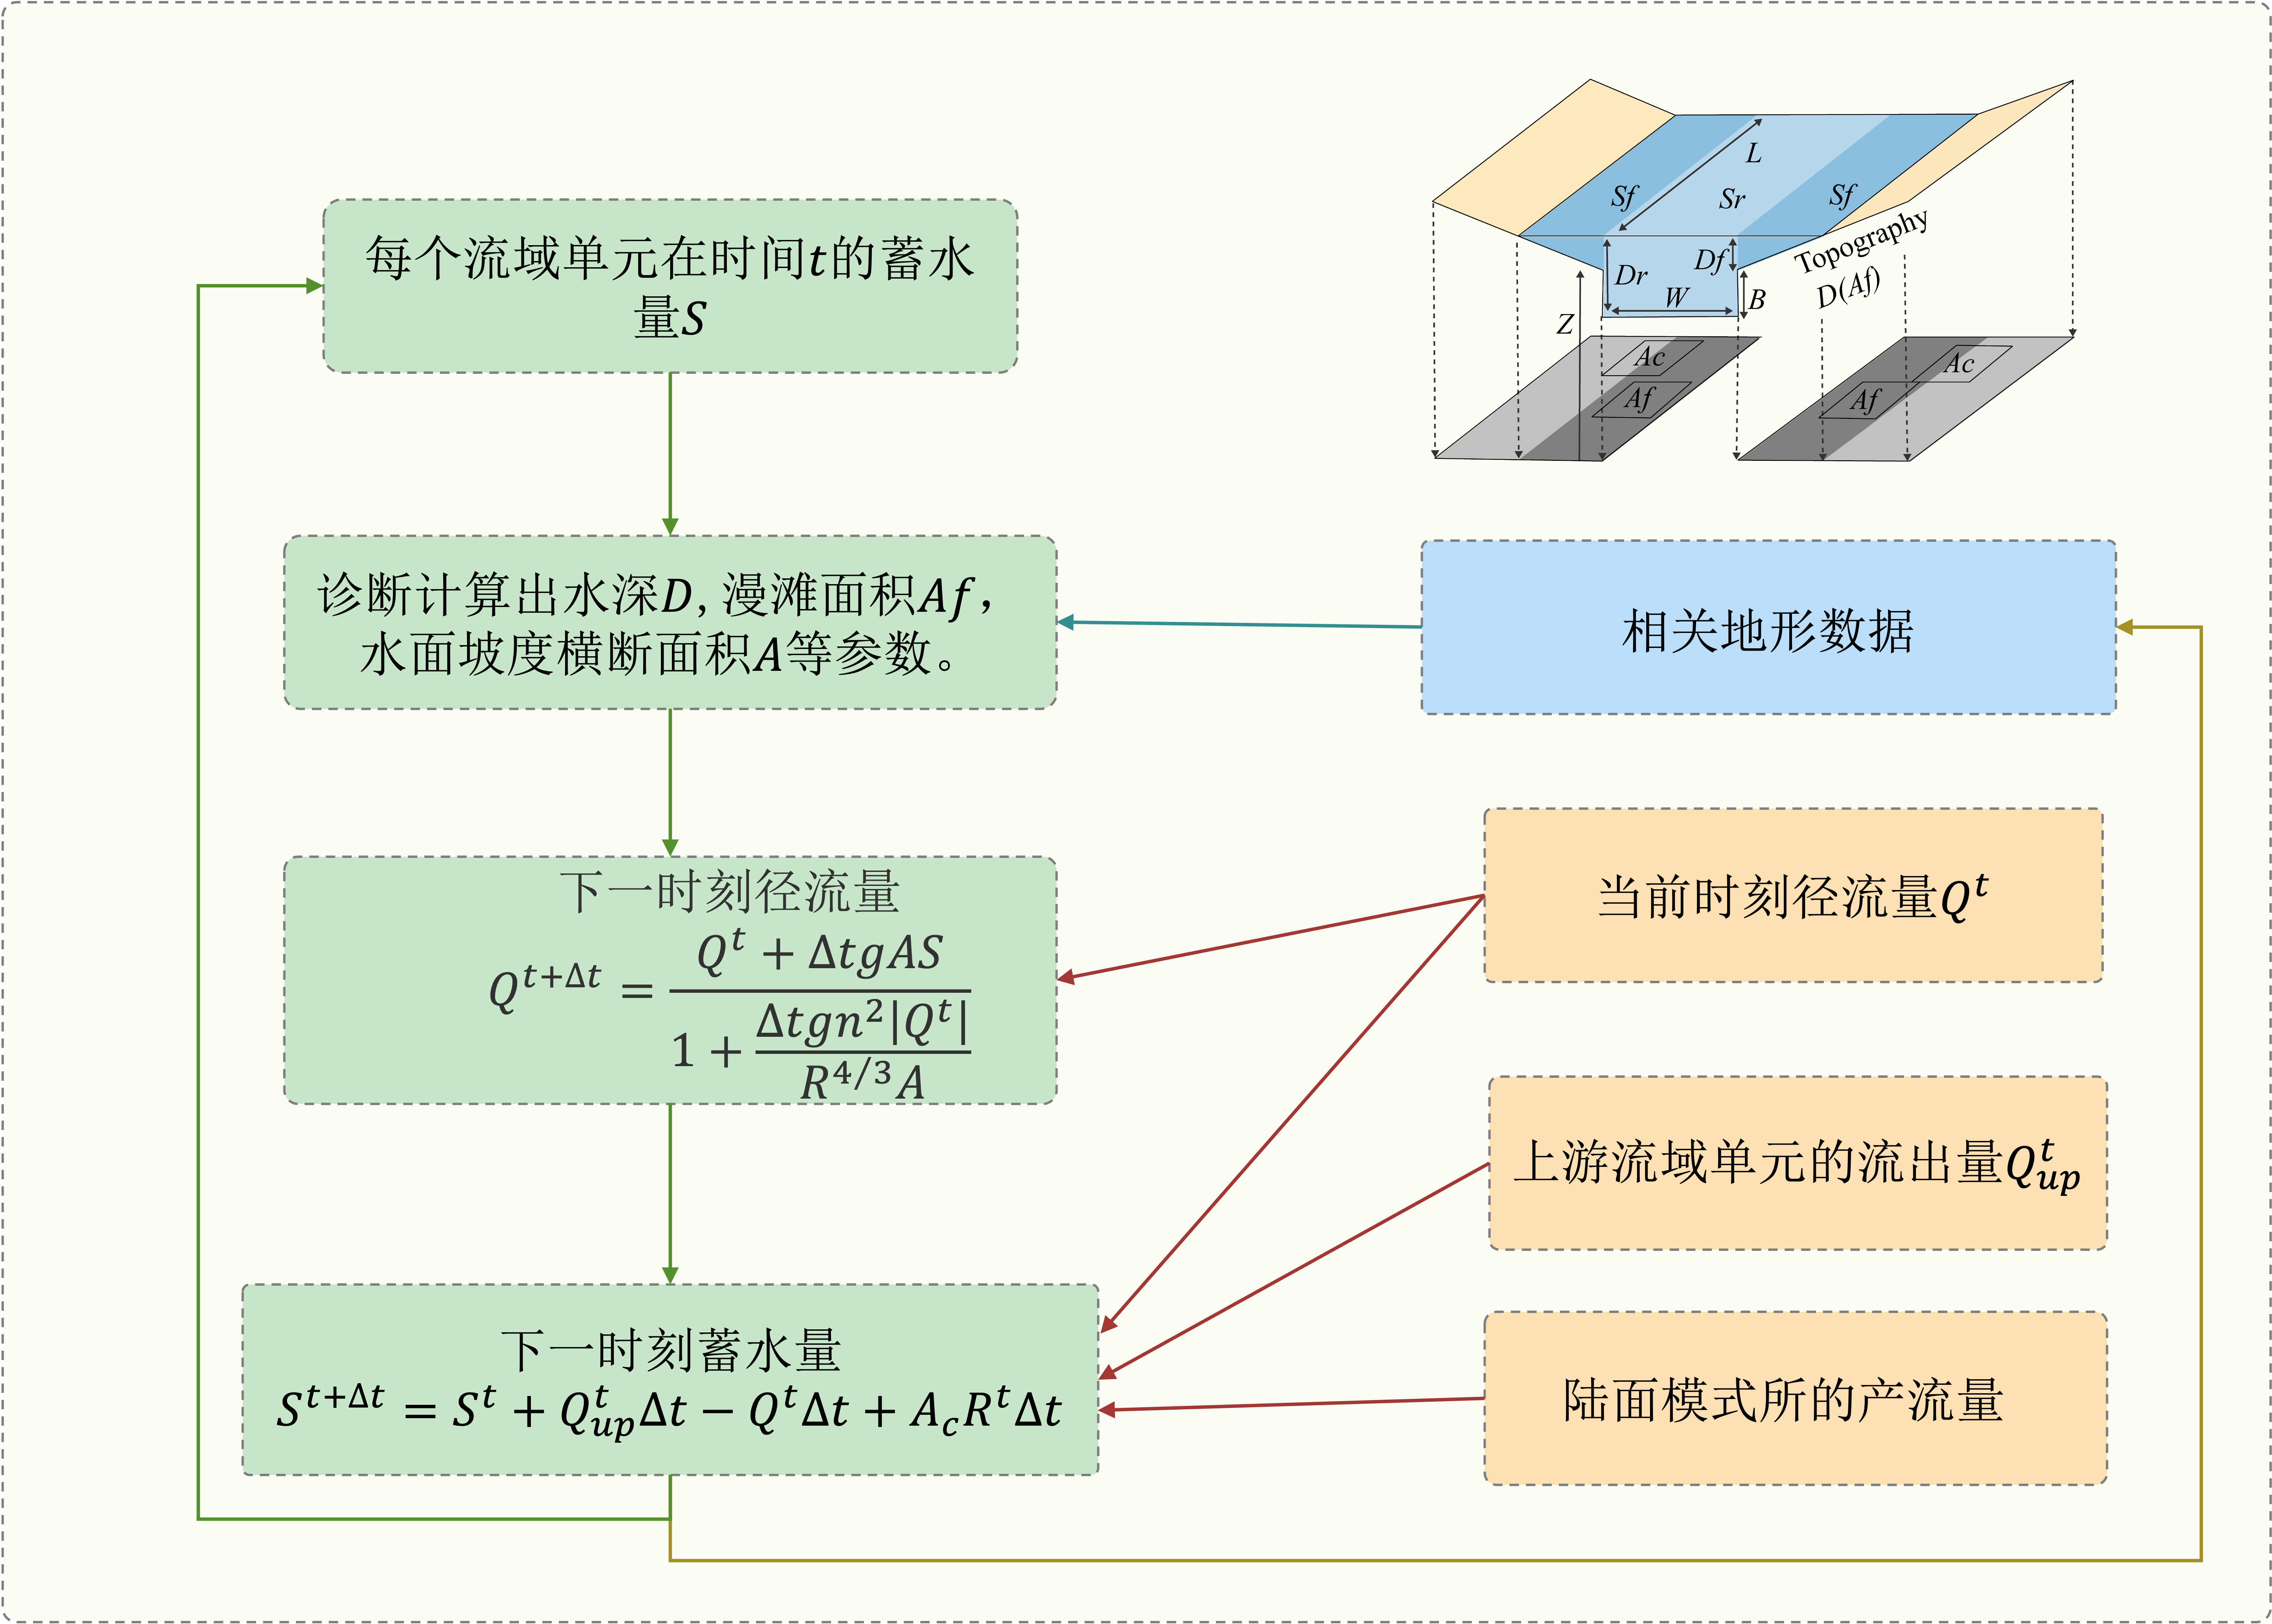
\includegraphics[width=0.8\textwidth]{Figures/陆地表面的水分循环/蓄水量变化计算流程图.png}
    \caption{CaMa-Flood~蓄水量变化计算流程图 }
    \label{fig:蓄水量变化计算流程图}
  \end{figure}
}
蓄水量随时间的变化的计算流程如图~\ref{fig:蓄水量变化计算流程图} 所示,指定流域单元的蓄水量变化的计算基于质量平衡方程:
\begin{equation}
  S_{i}^{t+\Delta t}=S_{i}^{t}+\sum_{k}^{Upstream} Q_{k}^{t} \Delta t-Q_{i}^{t} \Delta t+A c_{i} R_{i}^{t} \Delta t
\end{equation}
式中$S_{i}^{t}$和$S_{i}^{t+\Delta t}$分别代表单元$i$在时间$t$到时间$t+\Delta t$蓄水量的变化,$Q_i^t$代表在时间$t$该单元河流径流出流量 (河道内+漫滩),
$Q_k^t$代表在时间 $t$ 该单元从上游(upstream)网格($k$)接收的河流径流流入流量 (河道内+漫滩),$Ac_i$ 是单元$i$的面积,$R_i^t$ 代表流域单元 $i$ 的产流量。


\subsection{自适应时间步长的估算}
为避免固定时间步长计算所产生的数值振荡,提高数值方案稳定性,
CaMa-Flood 采用了~\citet{bates2010}提出的基于局部惯性方程并满足 Courant-Friedrichs-Lewy (CFL)
条件的自适应时间步长 ($DT_{\mathrm{adp}}$) 的估算方法:
\begin{equation}
  {DT}_{\max }={\alpha} \frac{\Delta x}{\sqrt{{\mathrm {g}} h_{\mathrm{t}}}}
\end{equation}
上式中$DT_{\mathrm{max}}$是最大可接受的时间步长,$\delta{x}$是该流域单元连接下游流域单元的河道长度 (river length) (\unit{m}),
$\alpha$是稳定性系数设为0.7,$h_{\mathrm {t}} $是该流域单元在时刻$t$的水流深度 (water depth) (\unit{m}),$\rm g$是重力加速度设为9.81 (\unit{m.s^{-2}})。
图~\ref{fig:自适应时间步长的估算} 展示了基于上述公式计算的某一时刻的$DT_{\mathrm{max}}$ (minute)。
在计算过程中,如果用户指定的默认时间步长$DT$大于$DT_{\mathrm{max}}$,则$DT$将被划分为满足$CFL$条件的更小的时间等分的时间步长$DT_{\mathrm{adp}}$;
如果用户指定的默认时间步长$DT$小于$DT_{\mathrm{max}}$,则实际计算步长按照用户指定的默认时间步长。

{
  \begin{figure}[htbp]
    \centering
    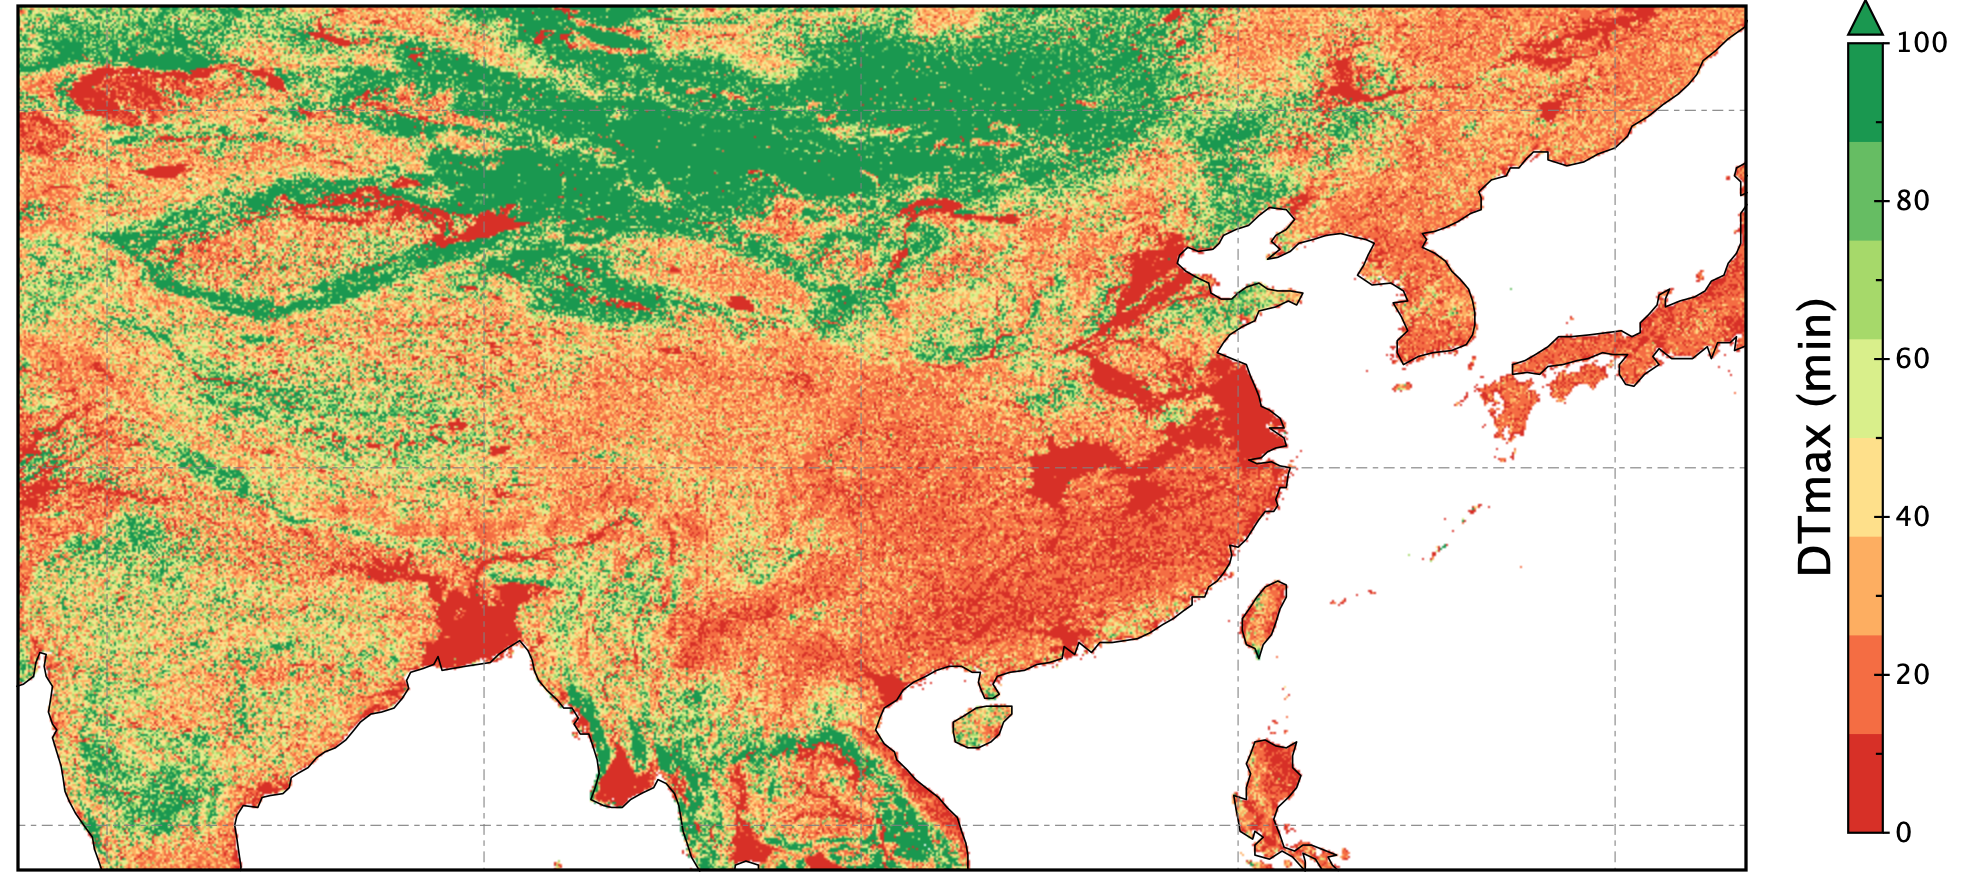
\includegraphics[width=0.8\textwidth]{Figures/陆地表面的水分循环/自适应时间步长的估算.png}
    \caption{CaMa-Flood自适应时间步长的估算案例}
    \label{fig:自适应时间步长的估算}
  \end{figure}
}
\subsection{双向耦合过程}
{
  \begin{figure}[htbp]
    \centering
    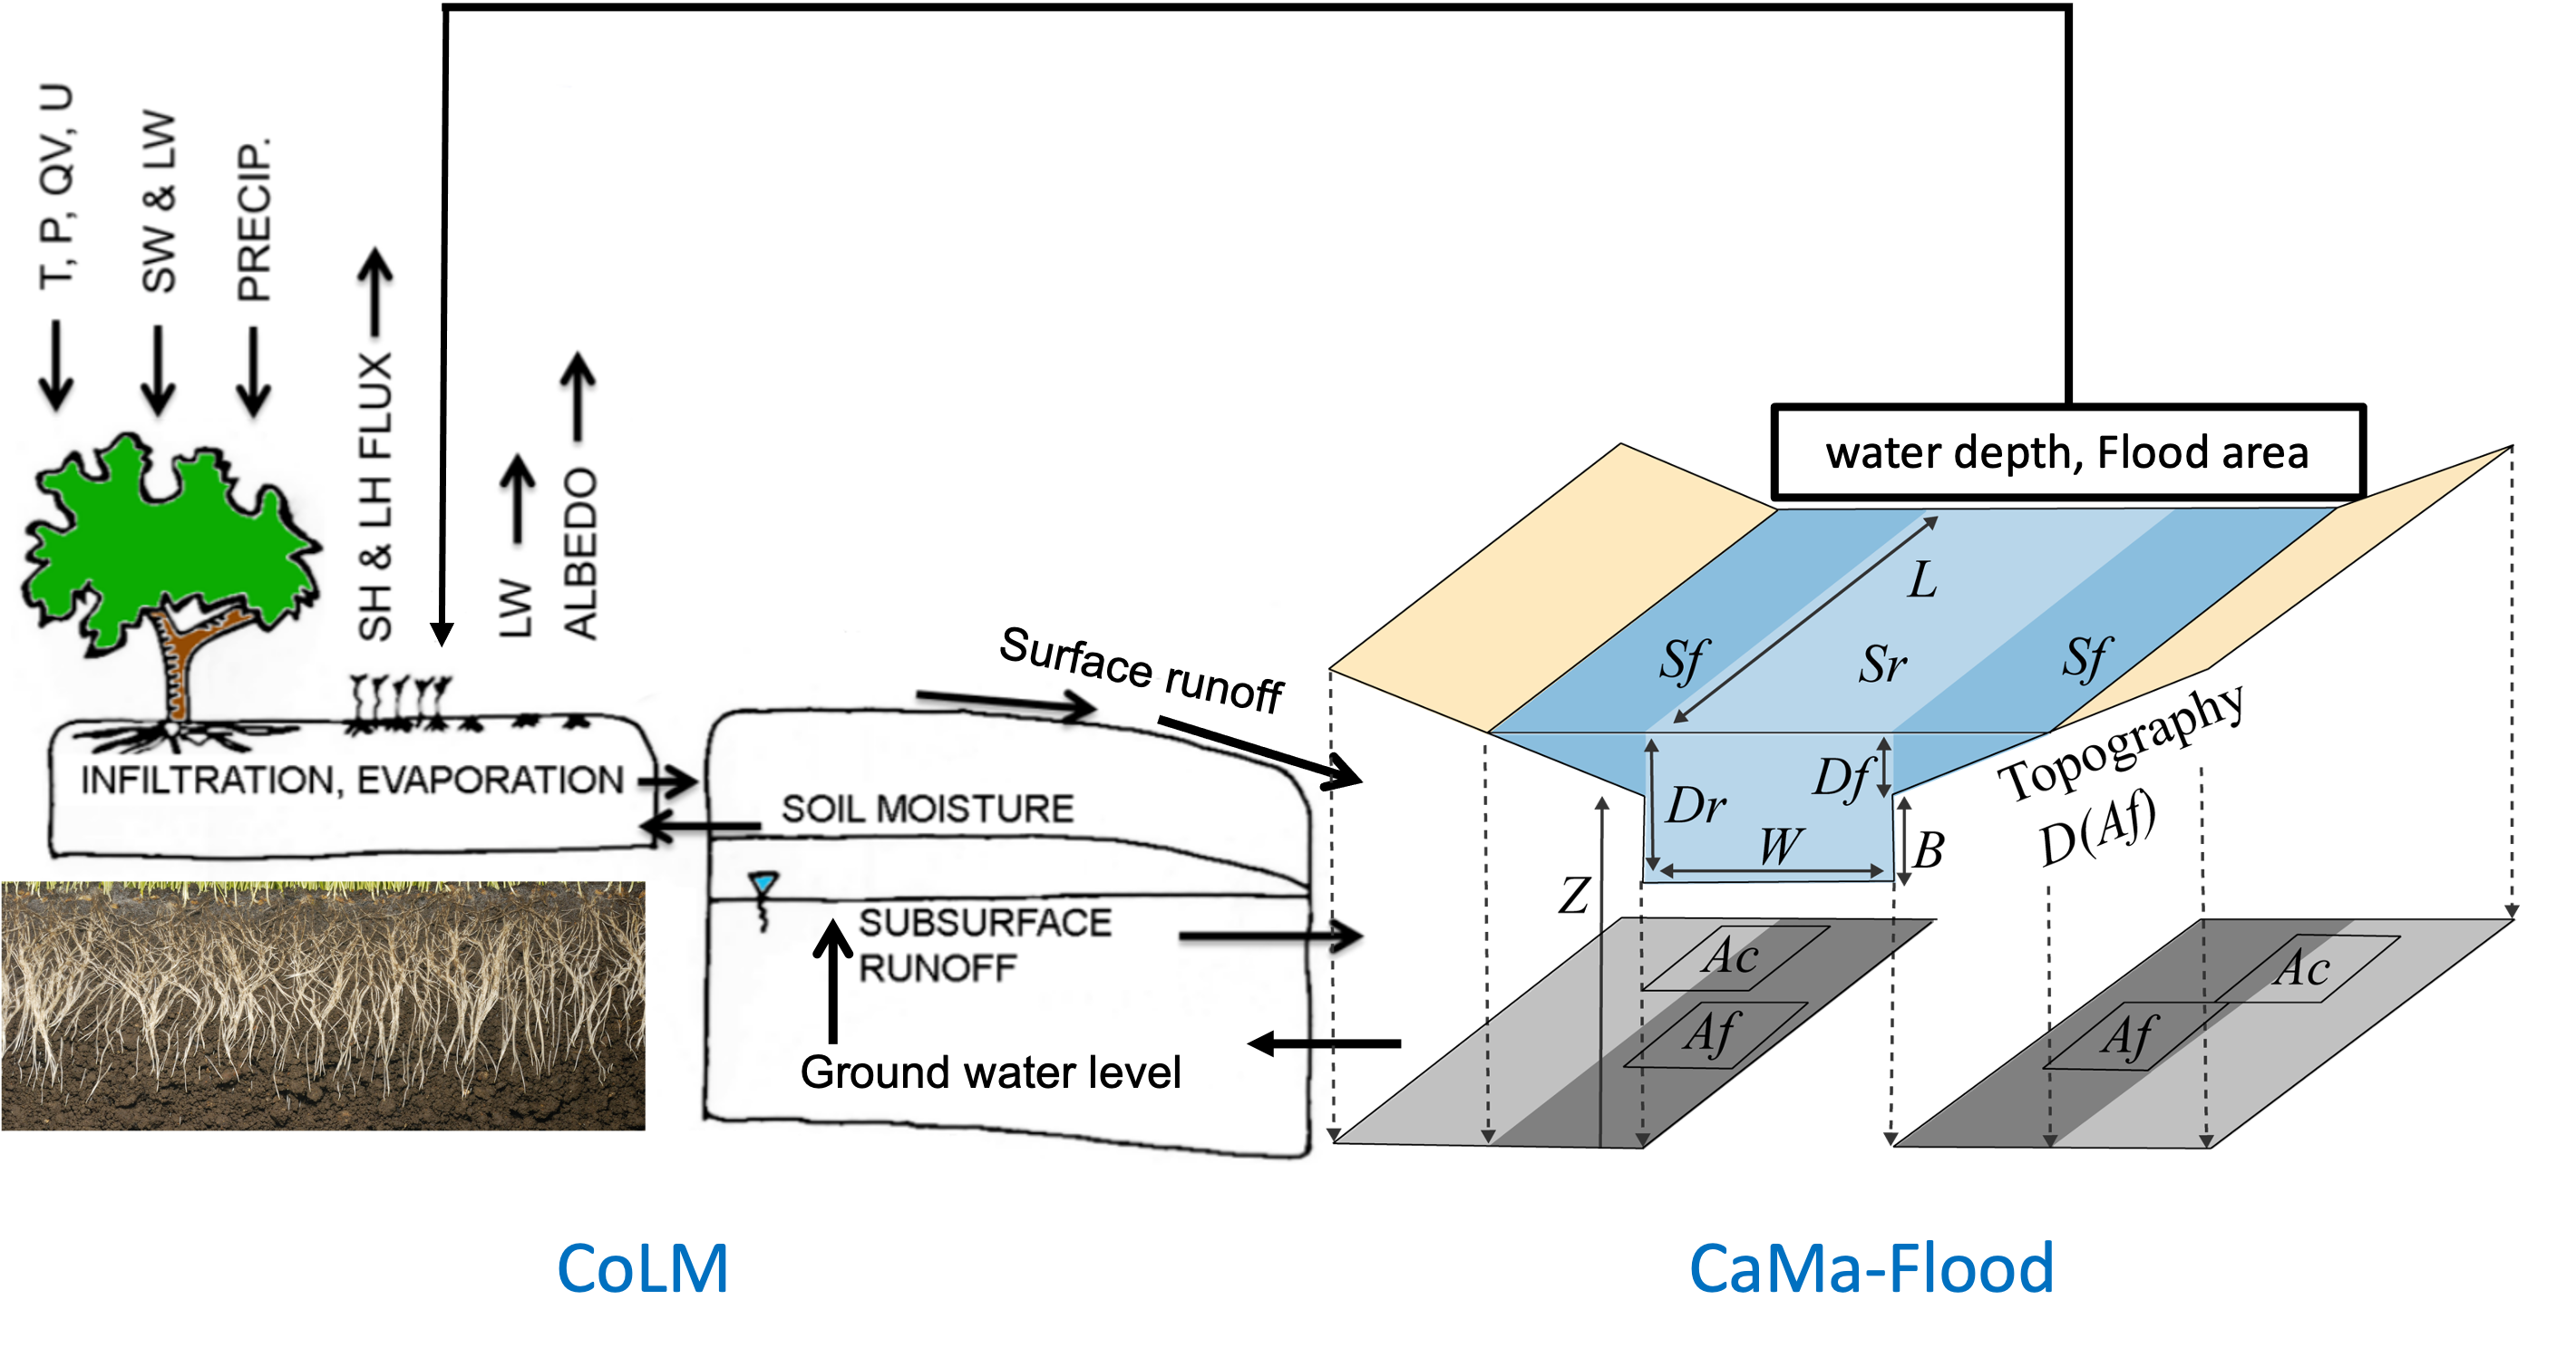
\includegraphics[width=0.8\textwidth]{Figures/陆地表面的水分循环/双向耦合.png}
    \caption{CaMa-Flood和CoLM双向耦合示意图}
    \label{fig:双向耦合}
  \end{figure}
}

CoLM 和CaMa-Flood已经实现了双向耦合,能够进行对水文过程的完整描述。如图~\ref{fig:双向耦合}所示,其耦合模拟包含一下过程:
\begin{enumerate}
  \item CoLM~模拟每个计算网格的地表能量平衡和地表水量平衡(融雪过程等)
  \item CoLM~模拟地表径流、各次表层的土壤含水量和地下水动态变化,并将土壤/地下水动态变化,并将运移结果分别反馈给~CoLM~和~CaMa-Flood~
  \item 通过接收CoLM的产流量,CaMa-Flood 计算河道径流、泛滥区域以及泛区水深,将是否发生洪水、洪水发生的区域、网格占比和洪水深度等相关结果反馈给CoLM
  \item 如果发生洪水,则在下一个时间步长、在非洪泛的网格占比,按原有的下垫面类型进行正常的~CoLM~模拟。而在洪水发生的网格占比,则将洪水深度作类似降水水量处理,并假设洪泛网格占比的下垫面为水面进行陆面状态模拟。最后再通过面积加权平均求出各类通量和状态变量
  \item 将加权平均后的下渗量和蒸发量传回给~CaMa-Flood,从总水量中扣除,更新水文水动力各项变量。

\end{enumerate}
